% -*- root: ../thesis.tex -*- 

\chapter{Design Pattern}
\label{ch:p02:ch02}

We design and implement a
\href{http://en.wikipedia.org/wiki/Sieve_of_Eratosthenes}{prime sieve
generator} using \href{https://github.com/CrispOSS/abs-api-parent}{ABS
API}. In this example, we strictly follow
\href{http://en.wikipedia.org/wiki/Object-oriented_programming}{object-oriented
design principles} and eventually mix in the actor model with the
implementation.

The following summarizes the prime sieve generation:

\begin{enumerate}
\itemsep1pt\parskip0pt\parsep0pt
\item
  The implementation works with a fixed input number \lstinline!N!.\\
\item
  The result is a sequence of prime numbers less than or equal to
  \lstinline!N!.\\
\item
  The implementation is required to be \emph{concurrent} and
  \emph{asynchronous}.
\end{enumerate}

The following diagram depicts a general structure of the prime sieve
generator in this example:

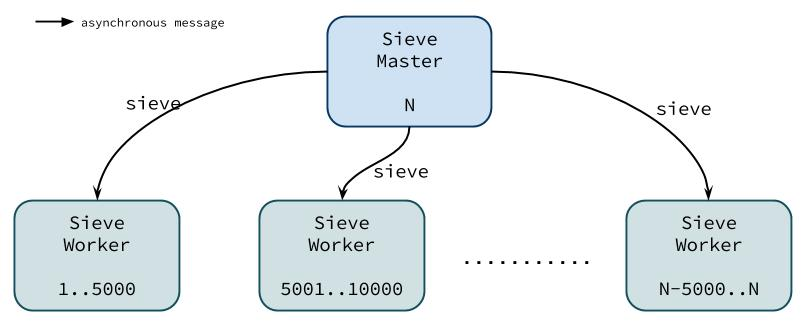
\includegraphics{figs/PrimeSieves.jpg}

\begin{itemize}
\itemsep1pt\parskip0pt\parsep0pt
\item
  \lstinline!SieveMaster! creates a number of buckets; i.e.
  \lstinline!SieveWorker!, each of which are responsible for a specific
  range.\\
\item
  The bucket size is chosen as \lstinline!5000! as a fixed number is
  this example.\\
\item
  \lstinline!SieveMaster! sends a message \lstinline!sieve! to all
  \lstinline!SieveWorker!s.\\
\item
  When a \lstinline!SieveWorker! finishes its computation it responds to
  the master by sending a message \lstinline!done!.\\
\item
  When the last worker is done, the prime generation completes.
\end{itemize}

Next, we design a Java interface for the prime sieves. Both
\lstinline!SieveMaster! and \lstinline!SieveWorker! are different
implementations of
\href{https://github.com/CrispOSS/prime-sieves/blob/master/src/main/java/com/github/crisposs/sieves/Sieve.java}{\lstinline!Sieve!}:

\lstset{language=Java}
\begin{lstlisting}[caption=Sieve Actor]
interface Sieve {
  void sieve();
  void done(List<Long> primes);
  Long last();
}
\end{lstlisting}

The above interface allows \lstinline!SieveMaster! to:

\begin{enumerate}
\itemsep1pt\parskip0pt\parsep0pt
\item
  break the input \lstinline!N! into a number of buckets\\
\item
  create a \lstinline!SieveWorker! for every bucket\\
\item
  initiate the algorithm with the first worker and moving on one by one
  when each worker is done\\
\item
  return \lstinline!last()! when the last worker finishes the
  computation
\end{enumerate}

The following presents the above steps in \lstinline!SieveWorker!'s
\lstinline!sieve()! method:

\begin{lstlisting}
SieveWorker w = getNextWorker() or finish
(M) send a message to `w` to `sieve`
\end{lstlisting}

and equivalently in \lstinline!SieveWorker!'s
\lstinline!done(List<Long> primes)! method:

\begin{lstlisting}
Collect generated `primes`
`sieve` again
\end{lstlisting}

When \lstinline!sieve()! in the master is done, the collected primes are
the generated prime numbers up to input \lstinline!N!.

The interesting part of the problem above in master's
\lstinline!sieve()! method is:

\begin{lstlisting}
(M) send a message to `w` to `sieve`
\end{lstlisting}

We model \emph{a message} by using

\begin{enumerate}
\itemsep1pt\parskip0pt\parsep0pt
\item
  \lstinline!java.lang.Runnable! to present a message with no interest
  in its return value\\
\item
  \lstinline!java.util.concurrent.Callable<V>! to present a message with
  a specific type of return value \lstinline!<V>!
\end{enumerate}

Through this model, we \textbf{separate} \emph{message delivery} from
\emph{message execution}. Essentially, a message execution is eventually
running the method invocation encapsulated in \lstinline!Runnable! or
\lstinline!Callable!.

For example:

\begin{enumerate}
\itemsep1pt\parskip0pt\parsep0pt
\item
  a message can be delivered in the same thread but executed in a
  different thread\\
\item
  a message can be delivered in a separate thread but executed in the
  same delivery thread\\
\item
  a message can be delivered in a separate thread and executed in a
  thread again different from the delivery thread
\end{enumerate}

The above models of message delivery and execution build the foundation
for \emph{synchronous} and \emph{asynchronous} message passing in ABS
API. By default, ABS API uses the 3rd approach in which all objects in
the runtime of the system share the same pool of threads.

We present \lstinline!(M)! in the following as:

\begin{lstlisting}[language=Java]
Runnable msg = new Runnable() {
  void run() {
    w.sieve();
  }
}
\end{lstlisting}

In Java 8, we can simply use
\href{https://docs.oracle.com/javase/tutorial/java/javaOO/lambdaexpressions.html}{Lambda
expressions}, so:

\begin{lstlisting}[language=Java]
Runnable msg = () -> w.sieve();
\end{lstlisting}

If we want to rewrite \lstinline!(M)! from the above:

\begin{lstlisting}[language=Java]
Runnable msg = () -> w.sieve();
send(w, msg);
\end{lstlisting}

in which \lstinline!send(Object, Object)! is expected to be a method
that semantically provides Approach 2 explained above to deliver the
message and execute it. Now the question is where
\lstinline!send(Object, Object)! can come from?

Next, let us zoom at \lstinline!SieveWorker!. A \lstinline!SieveWorker!
is also a \lstinline!Sieve! implementation a sketch of which can be
presented as:

\begin{lstlisting}
Sieve my range for prime numbers
(W) Reply to the "sender" with generated prime numbers
\end{lstlisting}

When a sieve worker has generated the prime numbers in its own range, it
is expected to reply back to the master. We designed
\lstinline!void done(List<Long>)! for this purpose in \lstinline!Sieve!.
We can rewrite \lstinline!(W)! from above as:

\begin{lstlisting}[language=Java]
List<Long> primes = // compute primes in my range
(W) Reply to master (sender) with message with invoking `done(primes)`
\end{lstlisting}

which means as before, we need to \emph{send a message} but the
difference here is that this is a \emph{reply message}. We can rewrite
then as:

\begin{lstlisting}[language=Java]
List<Long> primes = // compute primes in my range
Runnable replyMsg = () -> {
  (S) Sieve sender = sender();
  s.done(primes);
};
(R) reply(replyMsg);
\end{lstlisting}

We can \emph{functionally} define \lstinline!reply! in \lstinline!(R)!
as:

\begin{lstlisting}
reply = send(sender(), Object)
\end{lstlisting}

in which \lstinline!sender()! in \lstinline!(S)! refers to the
\emph{sender} object of the current message being processed by
\lstinline!this! object.

Naturally, we need to sketch the implementation of
\lstinline!done(List<Long>)! in \lstinline!SieveMaster! as it will be
the main receive of done messages:

\begin{lstlisting}[language=Java]
void done(List<Long> primes) {
  Store the primes
  sieve();
}
\end{lstlisting}

Simply, after each receipt of \lstinline!done!, the master stores the
newly generated primes and sieve again to see if there are still sieve
workers to do their computation.

We summarize the requirements that we have to be able to design this
example following both object-oriented design and asynchronous
computation:

\begin{itemize}
\itemsep1pt\parskip0pt\parsep0pt
\item
  \lstinline!send(Object o, Object msg)! sends a message \lstinline!msg!
  to an object \lstinline!o! in an asynchronous way\\
\item
  \lstinline!sender()! refers to the sender object of the currently
  being processed message in \lstinline!this! object\\
\item
  \lstinline!reply(Object msg)! send a message \lstinline!msg! as a
  reply to the \lstinline!sender()! of the processed message in
  \lstinline!this! object
\end{itemize}

This is where we mix object-oriented principles with Actor model brought
by ABS API. To add the above capabilities to our example, we simple
change \lstinline!Sieve! interface as:

\begin{lstlisting}[language=Java]
interface Sieve extends Actor {
}
\end{lstlisting}

to extend \lstinline!abs.api.Actor! interface. Now, all implementations
of \lstinline!Sieve! interface have access to the methods we draw as
expectations for this example. Applying the actor model API to this
sieve example as explained above can be depicted conceptually as:

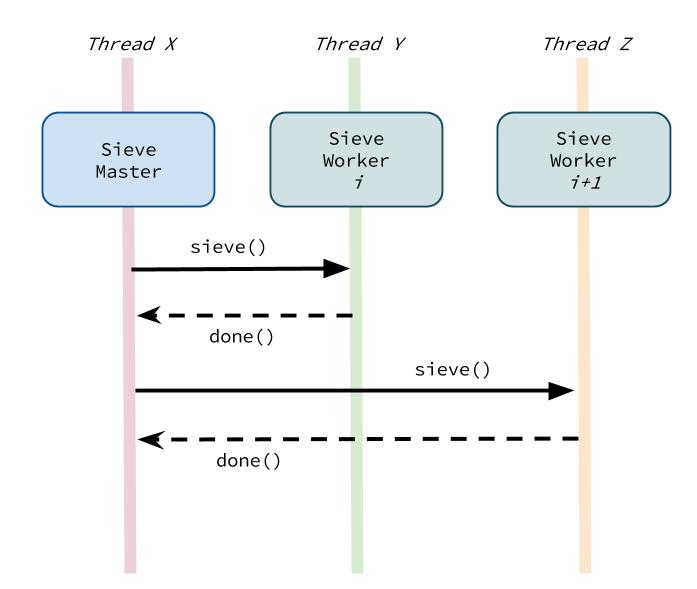
\includegraphics{figs/PrimeSievesControlFlow.jpg}

TODO: Generalize how we mixed the original object-oriented principles
and Actor model principles implemented in ABS API through Java 8.
